\documentclass{article}
\usepackage{amsmath, enumitem}
\usepackage{graphicx}
\usepackage{booktabs}
\usepackage{tabularx}
\usepackage[margin=1in]{geometry}
\usepackage{float}
\restylefloat{table}
\usepackage{placeins}
\usepackage{listings}

\usepackage{color}
 
\definecolor{codegreen}{rgb}{0,0.6,0}
\definecolor{codegray}{rgb}{0.5,0.5,0.5}
\definecolor{codepurple}{rgb}{0.58,0,0.82}
\definecolor{backcolour}{rgb}{0.95,0.95,0.92}
 
\lstdefinestyle{mystyle}{
    backgroundcolor=\color{backcolour},   
    commentstyle=\color{codegreen},
    keywordstyle=\color{magenta},
    numberstyle=\tiny\color{codegray},
    stringstyle=\color{codepurple},
    basicstyle=\footnotesize,
    breakatwhitespace=false,         
    breaklines=true,                 
    captionpos=b,                    
    keepspaces=true,                 
    numbers=left,                    
    numbersep=5pt,                  
    showspaces=false,                
    showstringspaces=false,
    showtabs=false,                  
    tabsize=2
}

\lstset{style=mystyle}

\begin{document}

\title{Econ 758 Homework 1}
\author{Ege Can, John Appert}
\maketitle

\section{Question 1}

\begin{enumerate}[label=\alph*]
\item Give a short description of the relevant aspects of the EITC expansion in 1993.(Hint: Have a look at Eissa and Hoynes, 2004.) Briefly discuss the theoretical predictions for the impact of the reform on the labor market participation of  single women with children. You do  not need  to present a formal model!

The earned income tax credit began as a reform to traditional welfare programs in that it requires the receipient to earn income in order to receive benefits.  This feature of the EITC was designed to counteract disincentives to work in traditional welfare programs.

There was an unintended effect from the program however.  While the program provides increasing benefits based on the number of children in a family, it was focused on household income.  This means that in a household where the mother is a secondary earner the choice to work is made after the husband's earnings are taken into account.  This feature results in the decision for a women to join the labor market to occur only if the husband has not maximized the benefit of EITC.  

In 1993 the EITC was modified to provide increased benefits to single parents.  In this case we would expect the impact single mothers to be significantly positive as we are increasing the benefit for them to work.

\item Would you expect the number of children to influence the size of the effect Why or why not? Explain.

Yes, we expect the number of children to impact the size of the effect.  The more children someone has the greater the benefit for entering the workforce.  Therefore, as the number of children increases we would expect a greater rise in the labor market participation rate.


\item  Generate a table with descriptive statistics (Table 1, structured as in Table I in Eissa and Liebman, 1996), which contains the sample means of the variables nonwhite age ed work  earn  for  two groups: single women with and without children. You do not need to display the  standard deviations. Briefly discuss the differences.

\item  Now calculate the sample means separately for single women with one child and women with two or m?ore children (add the information to Table 1). How do they differ from each other

\end{enumerate}

\section{Question 2}

For the following analysis you need to generate two dummy variables to identify the treatment group (single women with children) [call it child] and the post-treatment period (1994-1996) [call it post1993].

\begin{enumerate}[label=\alph*]
\item  Create a figure (Figure 1) that illustrates the annual mean labor market participation rates by year (1991-1996) for single women with children (treatment group) and single women without children (control group).Label the axes and include a title and a legend into the graph.


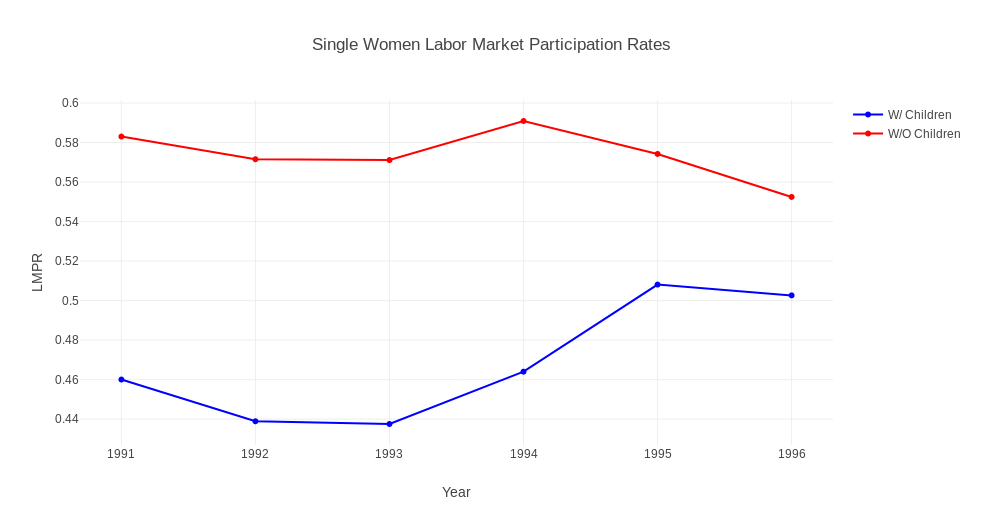
\includegraphics[width=5in, height=3in]{newplot}



\item Now normalize the value of the labor force participation rate for each of the two groups to group-specific 1991 values. That is, the mean of the labor  market participation rates in 1991 become equal to 1. Plot a graph (as the one before, including labeling, title, and legend) in Figure 2.



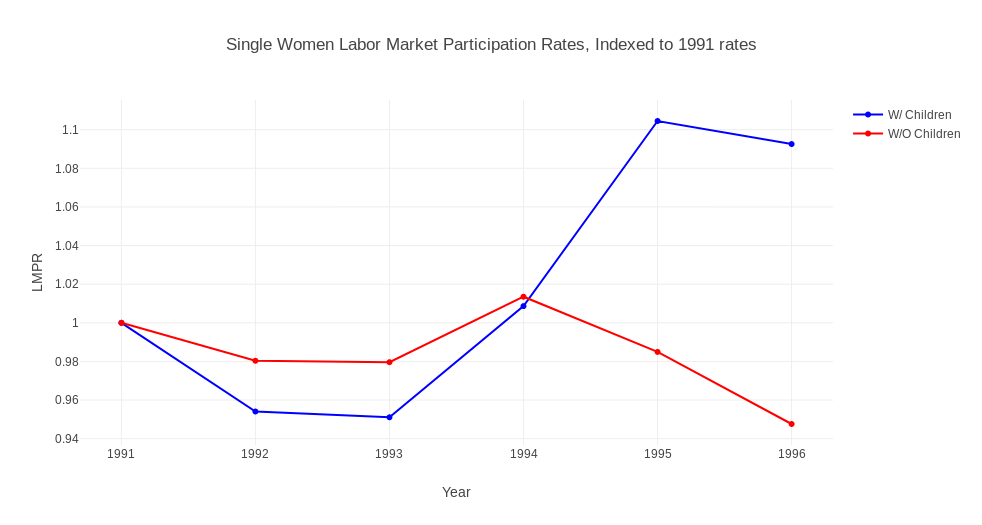
\includegraphics[width=5in, height=3in]{figure2}




\item  Based on Figures 1 and 2, discuss the validity of using single women without children as control group.

When looking at figure one it is difficult to determine whether or not the idea of using single women without children as a control group is valid.  The levels of labor market participation are significantly different and both trends seem similar.  However, once we index the labor market participation rate to 1991 and look at changes in the level with respect to 1991 we see that both groups track closely until 1994 when there is a divergence.  This implies that we can use single woment without children as a control group.

\item Calculate the sample means of labor force participation rates (work) of women with and without children for the pre-(average over 1991-1993) and post-reform (average over 1994-1996) period. Organize your table (Table 2) as in Table II in Eissa and Liebman (1996).



\begin{tabular}{ |p{2cm}||p{1cm}|p{1cm}|p{1cm}| p{1cm}|}
 \hline
 \multicolumn{5}{|c|}{Diff in Diff EITC Impact on Labor Supply} \\
 \hline
 Group  &Pre-1993&Post-1993 & Diff & Diff-in-Diff\\
 \hline
Treatment Group (Single Women With Children),  7819    &0.446 &0.491 &0.0448 & \\
\hline
Control Group (Single Women Without Children, 5927  & 0.575 & 0.573 & -0.002 & 0.0469 \\
\hline
Single Mother, One Child, 3058 &	0.524 &	0.554 & -0.127 &	\\
\hline
Control Group (Single Women Without Children),	5927 &	0.575 &	0.573 &	-0.002 &	-0.125 \\
\hline
Single Mother w/ Two Children, 4761 &	0.396 &	0.450 &	0.0532 &	\\
\hline
Control Group (Single Women Without Children), 5927 &	0.575 &	0.573 &	-0.002 &	0.055\\
\hline
\end{tabular}



\item Calculate the within-and between-group differences as well as the unconditional difference-in-differences estimate and add them to Table 2. Briefly comment on your results.

\item  Repeat the comparison separately for women with one child and for women with at least two children for the years before and after the EITC expansion. Again compute the within-and between-group differences and the difference-in-differences estimates. Compare each of the two groups separately to single women without children (the control group). Display the results in Table 3 and discuss your findings. For which of the two groups do you find larger treatment effects? Is this consistent with the theoretical predictions?

\item Return to the comparison of women with and without children. Estimate the difference-in-differences effect from the EITC expansion by running OLS regressions. As dependent variable, use the dummy indicating labor market participation(work). First run a regression without controls (“unconditional diff-in-diff estimate”). Then add control variables (urate nonwhite age ed) to obtain the “conditional diff-in-diff estimate”. Present your results (including standard errors) in Table 4 and interpret them. Compare the estimates and their statistical significance for the conditional and unconditional difference-in-differences estimates. Also comment on the estimated coefficients of child and post1993.

\begin{center}
\begin{tabular}{lclc}
\toprule
\textbf{Dep. Variable:}    &       work       & \textbf{  R-squared:         } &     0.013   \\
\textbf{Model:}            &       OLS        & \textbf{  Adj. R-squared:    } &     0.012   \\
\textbf{Method:}           &  Least Squares   & \textbf{  F-statistic:       } &     58.45   \\
\textbf{Date:}             & Wed, 20 Feb 2019 & \textbf{  Prob (F-statistic):} &  1.54e-37   \\
\textbf{Time:}             &     08:01:06     & \textbf{  Log-Likelihood:    } &   -9884.9   \\
\textbf{No. Observations:} &       13746      & \textbf{  AIC:               } & 1.978e+04   \\
\textbf{Df Residuals:}     &       13742      & \textbf{  BIC:               } & 1.981e+04   \\
\textbf{Df Model:}         &           3      & \textbf{                     } &             \\
\bottomrule
\end{tabular}
\begin{tabular}{lcccccc}
                  & \textbf{coef} & \textbf{std err} & \textbf{t} & \textbf{P$>$$|$t$|$} & \textbf{[0.025} & \textbf{0.975]}  \\
\midrule
\textbf{const}    &       0.5755  &        0.009     &    65.060  &         0.000        &        0.558    &        0.593     \\
\textbf{parent}   &      -0.1295  &        0.012     &   -11.091  &         0.000        &       -0.152    &       -0.107     \\
\textbf{Post1993} &      -0.0021  &        0.013     &    -0.160  &         0.873        &       -0.027    &        0.023     \\
\textbf{interact} &       0.0469  &        0.017     &     2.732  &         0.006        &        0.013    &        0.081     \\
\bottomrule
\end{tabular}
\begin{tabular}{lclc}
\textbf{Omnibus:}       &  5.965 & \textbf{  Durbin-Watson:     } &    1.934  \\
\textbf{Prob(Omnibus):} &  0.051 & \textbf{  Jarque-Bera (JB):  } & 2175.929  \\
\textbf{Skew:}          & -0.051 & \textbf{  Prob(JB):          } &     0.00  \\
\textbf{Kurtosis:}      &  1.054 & \textbf{  Cond. No.          } &     7.14  \\
\bottomrule
\end{tabular}
%\caption{OLS Regression Results}
\end{center}

Warnings: \newline
 [1] Standard Errors assume that the covariance matrix of the errors is correctly specified.


\begin{tabular}[H]{ |p{4cm}p{2cm}p{2cm}p{2cm}|}
 \hline
 \multicolumn{4}{|c|}{TABLE V} \\
 \multicolumn{4}{|c|}{OLS AND REDUCED-FORM ESTIMATES}\\
 \multicolumn{4}{|c|}{ OF EFFECT OF CLASS-SIZE ASSIGNMENT}\\
 \multicolumn{4}{|c|}{ AVERAGE PERCENTILE OF STANFORD ACHIEVEMENT TEST} \\
 \hline
 \hline
 \multicolumn{4}{|c|}{OLS Actual Class Size} \\
 \hline
 \multicolumn{4}{|c|}{A:Kindergarten} \\
 \hline
   Variable &(1) & (2) & (3) \\
 \hline

Small Class & 4.79&5.47&5.45 \\
&(0.901)&(1.456)&(1.394)\\
Regular Class with Aide&-.2742&-0.063&0.149 \\
&(0.839)&(1.33)&(1.29)\\
White/Asian (1=yes) &&&9.71\\
&-&-&(1.615)\\
Girl (1=yes)&&&4.64 \\
&-&-&(0.563)\\
Freelunch (1=yes)&&&-13.10 \\
&-&-&(0.934)\\
School Fixed Effects & No&Yes&Yes\\
\multicolumn{4}{|c|}{B:First Grade} \\
Small Class& 8.51&8.22&8.58\\
&(0.8)&(0.73)&(0.72)\\
Regular Class with Aide&3.44&2.07&1.96\\
&(0.77)&(0.69)&(0.68)\\
White/Asian (1=yes)&&&11.97\\
&-&-&(1.08)\\
Girl (1=yes)&&&3.34\\
&-&-&(0.56)\\
Free lunch (1=yes)&&&-5.59\\
&&&(0.68)\\
School Fixed Effects & No&Yes&Yes\\
\multicolumn{4}{|c|}{C:Second Grade} \\
Small Class& 5.91&6.49&6.58\\
&(0.85)&0.79)&(0.78)\\
Regular Class with Aide&1.43&1.76&1.69\\
&(0.81)&(0.73)&(0.72)\\
White/Asian (1=yes)&&&12.14\\
&-&-&(1.19)\\
Girl (1=yes)&&&3.34\\
&-&-&(0.60)\\
Free lunch (1=yes)&&&-2.14\\
&&&(0.78)\\
School Fixed Effects & No&Yes&Yes\\
\multicolumn{4}{|c|}{D:Third Grade} \\
Small Class& 5.31&5.47&5.36\\
&(0.86)&(0.81)&(0.81)\\
Regular Class with Aide&-0.47&-0.52&0.001\\
&((0.83)&(0.77)&(0.77)\\
White/Asian (1=yes)&&&11.88\\
&-&-&(1.27)\\
Girl (1=yes)&&&3.26\\
&-&-&(0.62)\\
Free lunch (1=yes)&&&0.66\\
&&&(0.85)\\
School Fixed Effects & No&Yes&Yes\\
\hline
\end{tabular}




\item Estimate a conditional (i.e., including urate nonwhite age ed), “placebo” treatment model on the pre-treatment period. For this purpose, take data from the years 1991-1993 only and leave the treatment and control groups unchanged. Assume for the analysis that the placebo reform would have taken place on January 1st, 1992 (generate a dummy variable postplacebo that is one for year 1992 and after and an interaction with child) and present your results (including standard errors) in Table 5. What do you find?

We find that when building a "placebo" model we find no significant effects on labor supply of single women with children in the period preceding the change in the EITC.  This supports the argument that the change we see in the later period is due to the changes in the EITC and not some other unobserved variable.  In this case we find the coefficient of the interaction variable is -0.0127 with a standard error of 0.024.


​
\begin{center}
\begin{tabular}{lclc}
\toprule
\textbf{Dep. Variable:}    &       work       & \textbf{  R-squared:         } &     0.031   \\
\textbf{Model:}            &       OLS        & \textbf{  Adj. R-squared:    } &     0.030   \\
\textbf{Method:}           &  Least Squares   & \textbf{  F-statistic:       } &     34.06   \\
\textbf{Date:}             & Wed, 20 Feb 2019 & \textbf{  Prob (F-statistic):} &  4.84e-47   \\
\textbf{Time:}             &     08:05:32     & \textbf{  Log-Likelihood:    } &   -5254.1   \\
\textbf{No. Observations:} &        7401      & \textbf{  AIC:               } & 1.052e+04   \\
\textbf{Df Residuals:}     &        7393      & \textbf{  BIC:               } & 1.058e+04   \\
\textbf{Df Model:}         &           7      & \textbf{                     } &             \\
\bottomrule
\end{tabular}
\begin{tabular}{lcccccc}
                  & \textbf{coef} & \textbf{std err} & \textbf{t} & \textbf{P$>$$|$t$|$} & \textbf{[0.025} & \textbf{0.975]}  \\
\midrule
\textbf{const}    &       0.5403  &        0.048     &    11.281  &         0.000        &        0.446    &        0.634     \\
\textbf{parent}   &      -0.1092  &        0.020     &    -5.490  &         0.000        &       -0.148    &       -0.070     \\
\textbf{Post1992} &      -0.0002  &        0.018     &    -0.009  &         0.993        &       -0.036    &        0.036     \\
\textbf{urate}    &      -0.0210  &        0.004     &    -4.750  &         0.000        &       -0.030    &       -0.012     \\
\textbf{nonwhite} &      -0.0394  &        0.012     &    -3.265  &         0.001        &       -0.063    &       -0.016     \\
\textbf{age}      &       0.0019  &        0.001     &     3.237  &         0.001        &        0.001    &        0.003     \\
\textbf{ed}       &       0.0157  &        0.002     &     7.103  &         0.000        &        0.011    &        0.020     \\
\textbf{interact} &      -0.0127  &        0.024     &    -0.525  &         0.599        &       -0.060    &        0.035     \\
\bottomrule
\end{tabular}
\begin{tabular}{lclc}
\textbf{Omnibus:}       &  0.010 & \textbf{  Durbin-Watson:     } &     1.968  \\
\textbf{Prob(Omnibus):} &  0.995 & \textbf{  Jarque-Bera (JB):  } &  1083.431  \\
\textbf{Skew:}          &  0.003 & \textbf{  Prob(JB):          } & 5.44e-236  \\
\textbf{Kurtosis:}      &  1.126 & \textbf{  Cond. No.          } &      328.  \\
\bottomrule
\end{tabular}
%\caption{OLS Regression Results}
\end{center}

Warnings: \newline
 [1] Standard Errors assume that the covariance matrix of the errors is correctly specified.


\end{enumerate}


\section{Code}

\lstinputlisting[language=Python]{python}

\end{document}

